%!TeX root=./ordenacao.tex

%% ------------------------------------------------------------------------- %%

\section{Lista Ordenada Cinética}
\label{lista:secao}
Um jeito natural de resolver o problema da lista ordenada cinética é
manter um vetor com os elementos da lista em ordem decrescente do
valor no instante atual.

Inicialmente o vetor começa com os valores dos elementos no instante
$t = 0$, ou seja, com o valor $x_0$ de cada elemento, e este vetor é
ordenado em ordem decrescente. Na verdade, o vetor pode armazenar
não os valores, mas os índices dos elementos, e fazemos ordenação
indireta. No caso de empates nos valores dos elementos, o desempate
será feito pela velocidade, ou seja, se dois elementos, digamos $i$
e $j$, possuem o mesmo valor $x_0$, mas a velocidade de $i$ é maior
que a de $j$, então $i$ será tratado como se possuísse maior valor
que $j$ no instante inicial. Esse mesmo critério de desempate será
aplicado em todos os instantes e também em todos os problemas daqui
em diante.

Uma vez de posse do vetor ordenado com os valores iniciais
decrescentemente, construímos um certificado para cada par de
elementos consecutivos no vetor. O $i$-ésimo certificado, denotado
pelo par $(i, t)$, se refere ao par das posições $i$ e $i + 1$. O
valor $t$ consiste no instante de tempo em que o $i$-ésimo elemento
deixará de ter um valor maior que o valor do $(i + 1)$-ésimo
elemento do vetor, se esse instante for maior ou igual a 0, ou em
geral ao instante atual. Do contrário, o valor $t$ consiste em
$+\infty$. O valor $t$ do certificado é o seu \underline{prazo de
validade}.

Esses prazos de validade determinam os \underline{eventos} que
potencialmente causarão modificações no vetor que mantém os
elementos ordenados pelo seu valor e consequentemente em alguns
certificados.

Esses $n - 1$ certificados são colocados em uma fila com
prioridades, com o prazo de validade determinando a prioridade.
Estamos interessados nos certificados com menor prazo de validade.
Ou seja, a fila com prioridades pode ser implementada com um heap de
mínimo que usa os prazos de validade como chave.

Para descrever a implementação das três operações, precisamos
estabelecer o nome das variáveis usadas. São elas:
\begin{enumerate}
    \item $n$: o número de elementos dados;
    \item $x_0$ e \textit{speed}: vetores com o valor e a
    velocidade inicial de cada um dos $n$ elementos;
    \item \now: instante atual;
    \item \textit{sorted}: vetor com os índices dos $n$
    elementos em ordem decrescente do seu valor no instante
    \textit{now};
    \item \textit{indS}: vetor de $n$ posições; \textit{indS}[$i$]
    guarda a posição em \textit{sorted} do elemento $i$;
    \item \textit{cert}: vetor com os $n-1$ certificados;
    \textit{cert}$[i]$ guarda o certificado entre $\sorted[i]$ e
    ${\sorted[i+1]}$, para~$1~\leq~i~<~n$;
    \item \textit{Q}: fila com prioridades para os certificados.
\end{enumerate}

A interface da fila com prioridades que utilizaremos inclui as duas
seguintes operações:
\begin{enumerate}
    \item \textsc{minPQ}$(Q)$: devolve o certificado $(i, t)$
    com chave $t$ mínima em $Q$;
    \item \textsc{updatePQ}$(Q, i, t)$: altera a chave do
    $i$-ésimo certificado para $t$ e ajusta $Q$ de acordo.
\end{enumerate}
O vetor $\textit{indS}$ nos permite implementar a operação
\textsc{change} de maneira eficiente, pois, dado um elemento $j$,
precisamos saber a posição $i$ do elemento $j$ em $\sorted$ para
recalcular os certificados relacionados com a posição $i$.

Para implementar a operação \textsc{updatePQ}$(Q, i, t)$ em tempo
logarítmico no número de elementos na fila $Q$, é necessário
utilizar um vetor adicional \textit{indQ} que guarda em
\textit{indQ}$[i]$ a posição do $i$-ésimo certificado em $Q$.

Com isso, a operação \textsc{advance}$(t)$ segue uma ideia bem
simples: enquanto $t$ for maior que o prazo de validade do próximo
evento, avançamos \textit{now} para esse prazo de validade e
tratamos esse evento. Nos problemas seguintes, a operação
\textsc{advance}$(t)$ será sempre a mesma; as únicas mudanças
ocorrerão no tratamento de um evento. Um evento está associado a um
certificado $(i, t)$ que expira quando $\now = t$. O tratamento do
evento correspondente ao certificado $(i, t)$ consiste em trocar de
lugar os índices das posições $i$ e $i + 1$ do vetor
\textit{sorted}, recalcular o prazo de validade do $(i-1)$-ésimo
certificado se $i > 1$, e do $(i + 1)$-ésimo certificado se $i < n -
1$. O $i$-ésimo certificado também deve ser ajustado para $+\infty$.
Finalmente, é necessário fazer ajustes em $Q$, alterando a chave dos
certificados que sofreram alteração.

\begin{algorithm}[H]
    \caption[Algoritmo \textsc{advance}]{Função \textsc{advance}.} \label{alg:lista-ordenada:advance}
\begin{algorithmic}[1]
    \Function{advance}{$t$}
        \If{$t < $ \now}
            \State \Return
        \EndIf
        \State $i \leftarrow \Call{minPQ}{$Q$}$
        \While{$t \geq$ \cert[$i$]}
            \State \now $~\leftarrow$ \cert[i]
            \State $\Call{event}$
            \State $i \leftarrow \Call{minPQ}{$Q$}$
        \EndWhile
        \State \now $~\leftarrow$ $t$
    \EndFunction
\end{algorithmic}
\end{algorithm}

Na implementação da operação \textsc{event}, utilizaremos a rotina
\textsc{update}$(i)$ para calcular a nova validade $t$ do $i$-ésimo
certificado, se $1 \leq i < n$, e fazer os devidos ajustes em $Q$.
Para calcular $t$, utilizaremos uma rotina chamada
\textsc{expire}$(i, j)$, que calcula a validade dos certificados
entre os elementos $i$ e $j$. A rotina auxiliar \textsc{expire}$(i,
j)$ não mudará para outros problemas, mantendo a mesma definição.

\begin{algorithm}
    \caption{Função \textsc{update}.} \label{lista:update}
\begin{algorithmic}[1]
    \Function{update}{$i$}
        \If{$1 \leq i < n$}
            \State $t \leftarrow $ \Call{expire}{$i,i+1$}
            \State \Call{updatePQ}{$Q,i,t$}
        \EndIf
    \EndFunction
\end{algorithmic}
\end{algorithm}

\begin{algorithm}
    \caption{Função \textsc{event}.} \label{torneioi:evento}
    \begin{algorithmic}[1]
        \Function{event}{\nnull}
            \State $e \leftarrow  $ \Call{minPQ}{$Q$}
            \While{$e.\cert$ = \now}
                \State $j \leftarrow e.\lastmatch$
                \State $k \leftarrow 2\cdot \floor{\frac{j}{2}}
                + ((j + 1)\mod2)$ \Comment{adversário}
                \While{$j > 1$ \AND \Call{compare}{$j, k$}}
                    \State \torneio[$\floor{\frac{j}{2}}$]
                    $\leftarrow~$\torneio[$j$]
                    \State $\torneio[k].\lastmatch$ $\leftarrow k$
                    \State \Call{update}{$\torneio[k]$}
                    \State $j \leftarrow \floor{\frac{j}{2}}$
                    \State $k \leftarrow 2\cdot \floor{\frac{j}{2}}
                    + ((j + 1)\mod2)$ \Comment{adversário}
                \EndWhile
                \State $\torneio[j].\lastmatch \leftarrow j$
                \State \Call{update}{$\torneio[j]$}
                \State $e \leftarrow  $ \Call{minPQ}{$Q$}
            \EndWhile
        % \LineComment{swapHeap$(i, \floor{\frac{i}{2}})$ troca \heap[$i$] por \heap$\left[\floor{\frac{i}{2}}\right]$}
        \EndFunction
        \LineComment{\Call{compare}{$i, j$} retorna se o valor
        de $i$ é maior que o valor de $j$.}
    \end{algorithmic}
\end{algorithm}

As figuras \ref{fig:lista:expire} e \ref{fig:lista:update} ilustram
o tratamento do evento de expiração do segundo certificado.

\begin{figure}
    \centering
    \begin{tikzpicture}[thick, scale=0.8]
        \node[label={1},circle,draw,minimum size=1cm]
            (1) at (0,0) {$3$};
        \node[label={2},circle,draw,minimum size=1cm]
            (2) at (-4,-2) {$3$};
        \node[label={3},circle,draw,minimum size=1cm]
            (3) at (4,-2) {$4$};
        \node[label={4},circle,draw,minimum size=1cm]
            (4) at (-6,-4) {$1$};
        \node[label={5},circle,draw,minimum size=1cm]
            (5) at (-2,-4) {$3$};
        \node[label={6},circle,draw,minimum size=1cm]
            (6) at (2,-4) {$4$};
        \node[label={7},circle,draw,minimum size=1cm]
            (7) at (6,-4) {$6$};
        \node[label={8},circle,draw,minimum size=1cm]
            (8) at (-7,-6) {$8$};
        \node[label={9},circle,draw,minimum size=1cm]
            (9) at (-5,-6) {$1$};
        \node[label={10},circle,draw,minimum size=1cm]
            (10) at (-3,-6) {$2$};
        \node[label={11},circle,draw,minimum size=1cm]
            (11) at (-1,-6) {$3$};
        \node[label={12},circle,draw,minimum size=1cm]
            (12) at (1,-6) {$4$};
        \node[label={13},circle,draw,minimum size=1cm]
            (13) at (3,-6) {$5$};
        \node[label={14},circle,draw,minimum size=1cm]
            (14) at (5,-6) {$6$};
        \node[label={15},circle,draw,minimum size=1cm]
            (15) at (7,-6) {$7$};
        \node[label={16},circle,draw,minimum size=1cm]
            (16) at (-8,-8) {$8$};
        \node[label={17},circle,draw,minimum size=1cm]
            (17) at (-6,-8) {$9$};

        \draw[thick] (1) -- (2);
        \draw[<-,line width=\thickness, red] (2) -- (4);
        \draw[<-,thick, dashed, red] (4) -- (8);
        \draw[thick] (4) -- (9);
        \draw[thick] (8) -- (16);
        \draw[<-,line width=\thickness, red] (8) -- (17);
        \draw[thick] (2) -- (5);
        \draw[<-,line width=\thickness, red] (5) -- (10);
        \draw[thick] (5) -- (11);
        \draw[<-,line width=\thickness, red] (1) -- (3);
        \draw[thick] (3) -- (6);
        \draw[<-,line width=\thickness, red] (3) -- (7);
        \draw[thick] (6) -- (12);
        \draw[<-,line width=\thickness, red] (6) -- (13);
        \draw[thick] (7) -- (14);
        \draw[<-,line width=\thickness, red] (7) -- (15);
    \end{tikzpicture}
    \caption[Representação de certificado expirado]{cert[$8$] expirou.}
    \label{fig:torneio:evento}
\end{figure}

\begin{algorithm}
    \caption{Função \textsc{update}.} \label{lista:update}
\begin{algorithmic}[1]
    \Function{update}{$i$}
        \If{$1 \leq i < n$}
            \State $t \leftarrow $ \Call{expire}{$i,i+1$}
            \State \Call{updatePQ}{$Q,i,t$}
        \EndIf
    \EndFunction
\end{algorithmic}
\end{algorithm}

\begin{algorithm}
    \caption{Função \textsc{query\_kth}.} \label{lista:query}
\begin{algorithmic}[1]
    \Function{query\_kth}{$i$}
        \If{$1 \leq i \leq n$}
            \State \Return \sorted[$i$]
        \EndIf
        \State \Return $-1$
    \EndFunction
\end{algorithmic}
\end{algorithm}

\begin{algorithm}
    \caption{Função \textsc{change}.} \label{torneioi:change}
    \begin{algorithmic}[1]
        \Function{change}{$j, v$}
            \State $e \leftarrow$ \Call{getObject}{$j$}
            \State $e.x_0 \leftarrow e.x_0+~(e.\speed -~v)~\cdot~\now$;
            \State $e.\speed \leftarrow v$
            \State $i \leftarrow e.\lastmatch$
            \State \Call{update}{$e$}
            \While{$i < n$}
                \If{$\torneio[i] = \torneio[2i]$}
                    \State $i \leftarrow 2i$
                \Else
                    \State $i \leftarrow 2i + 1$
                \EndIf
                \State $k \leftarrow 2\cdot \floor{\frac{i}{2}}
                + ((i + 1)\mod2)$ \Comment{adversário}
                \State \Call{update}{$\torneio[k]$}
            \EndWhile
        \EndFunction
    \end{algorithmic}
\end{algorithm}

A operação \textsc{query\_kth}$(i)$ consiste em devolver
\textit{sorted}$[i]$, enquanto que a operação \textsc{change}$(j,
v)$ consiste em alterar a posição $x_0[j]$ para $x_0[j] +
(\mathit{speed}[j] - v)\cdot now$, a posição \textit{speed}[j] para
\textit{v} e recalcular os eventuais certificados de que $j$
participa. O novo valor da posição $x_0[j]$ corresponde à posição
inicial do elemento caso ele tivesse começado com essa velocidade e
estivesse na posição atual agora. Para tanto, a partir da posição
$i$ em que $j$ se encontra no vetor \textit{sorted}, podemos
recalcular \textit{cert}$[i - 1]$ se $i > 1$ e \textit{cert}$[i]$ se
$i < n$, como ilustrado na figura \ref{fig:lista:after}, acionando
a rotina \textsc{updatePQ} para fazer os devidos acertos em~$Q$
correspondentes a estas modificações.

\begin{figure}[H]
    \centering
    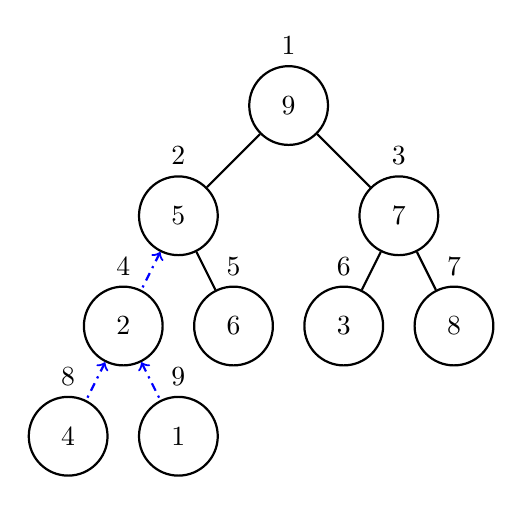
\begin{tikzpicture}[thick, scale=0.7]
        \node[label={1},circle,draw,minimum size=1cm]
        (1) at (0,0) {$9$};
        \node[label={2},circle,draw,minimum size=1cm]
        (2) at (-2,-2) {$5$};
        \node[label={3},circle,draw,minimum size=1cm]
        (3) at (2,-2) {$7$};
        \node[label={4},circle,draw,minimum size=1cm]
        (4) at (-3,-4) {$2$};
        \node[label={5},circle,draw,minimum size=1cm]
        (5) at (-1,-4) {$6$};
        \node[label={6},circle,draw,minimum size=1cm]
        (6) at (1,-4) {$3$};
        \node[label={7},circle,draw,minimum size=1cm]
        (7) at (3,-4) {$8$};
        \node[label={8},circle,draw,minimum size=1cm]
        (8) at (-4,-6) {$4$};
        \node[label={9},circle,draw,minimum size=1cm]
        (9) at (-2,-6) {$1$};

        \tikzstyle{cert}=[<-, dashdotted, blue, thick]
        \draw[thick] (1) -- (2);
        \draw[thick] (1) -- (3);
        \draw[cert] (2) -- (4);
        \draw[thick] (2) -- (5);
        \draw[thick] (3) -- (6);
        \draw[thick] (3) -- (7);
        \draw[cert] (4) -- (8);
        \draw[cert] (4) -- (9);
    \end{tikzpicture}
    \caption[Exemplo certificados do heap cinético após operação \textsc{change}]{Após a mudança de
    velocidade do elemento 2, que se encontra em \heap[$4$], os certificados
    \cert[$4$], \cert[$8$] e \cert[$9$] foram atualizados.}
    \label{fig:predeventheap}
\end{figure}
